\chapter{Related Works}
Categorization is not a new topic, nor is taking advantage of Wikipedia in a categorization process. There are many papers about the topic, and we did some research to avoid problems already solved by others and to get inspiration for our project. This chapter is dedicated to projects with related topics. It starts by giving a short introduction to the projects we have studied.
The  projects concerned with Wikipedia's category structure is covered in \ref{sec:category_structure}, while section \ref{sec:extracting_keywords} is dedicated to the process of extracting keywords from Wikipedia. 
%The process of extracting keywords from Wikipedia is covered in section \ref{sec:extracting_keywords}, while section   is dedicated to projects concerned with Wikipedia's category structure. 
Section \ref{sec:classifiers_based_on_wikipedia} covers classifiers based on Wikipedia, including the evaluation of the classifiers studied. Finally, section \ref{sec:disambiguation} gives an introduction to different types of disambiguation in NLP and reviews projects for solving disambiguation. 

\begin{comment}

, before it covers two tasks within the implementation; \emph{extracting keywords} and \emph{deciding content of Wikipedia articles based on the category structure}. Section \ref{sec:disambiguation} is dedicated to different approaches for solving ambiguous words and phrases which is one of the most discussed problems in NLP. Finally, the chapter reviews different approaches of evaluating the classifier and reviews some of the results found in other projects. 

%Some of the projects have also given useful help in the task of deciding on approaches 



\begin{comment}
Extracting Semantic Relationships between Wikipedia Categories
    - chernov2006extracting
Identifying document topics using the Wikipedia category network: 

All Our N-Gram are Belong to You: Encknowledge
Overcoming the Brittleness Bottleneck using Wikipedia: Enhancing Text Categorization with Encyclopedic Knowledge: brittleness
Entity Extraction, Linking, Classification, and Tagging for Social Media: A Wikipedia-based Approach: entityextraction
Large-Scale Taxonomy Mapping for Restructuring and Integrating Wikipedia: ponzetto2009large
Automatic ontology extraction for document classification: kozlova2005automatic

named entity disambiguation by leveraging wikipedia semantic knowledge: han2009named
large-scaled named entity disambiguation based on Wikipedia data: cucerzan2007large

decoding wikipedia categories for knowledge adcquistion: nastase2008decoding
\end{comment}

%\section{Disambiguation}
%\label{sec:disambiguation}

\begin{comment}
De ulike prosjektene: 

Projects with classifier creation: 

Projects determining content based on keyword extraction:
-Entity Extraction, Linking, Classification, and Tagging for Social Media: A Wikipedia-based Approach: entityextraction
-Large-Scale Taxonomy Mapping for Restructuring and Integrating Wikipedia: ponzetto2009large
-Automatic ontology extraction for document classification: kozlova2005automatic
-Overcoming the Brittleness Bottleneck using Wikipedia: Enhancing Text Categorization with Encyclopedic Knowledge: brittleness
-Wikify!: linking documents to encyclopedic knowledge: mihalcea2007wikify


Projects for determining content based on the category structure

Taking advantage of the category structure: 
-Extracting Semantic Relationships between Wikipedia Categories: chernov2006extracting
-Identyfing document topics using the Wikipedia category network: schonhofen2009identifying
-decoding wikipedia categories for knowledge adcquistion: nastase2008decoding

Disambiguation:
-named entity disambiguation by leveraging wikipedia semantic knowledge: han2009named
-large-scaled named entity disambiguation based on Wikipedia data: cucerzan2007large
-Distributed representations of words and phrases and their compositionality: mikolov2013distributed


% What??? All Our N-Gram are Belong to You: Encknowledge

\end{comment}

\section{Similar Projects}
\label{sec:similar_projects}
Several projects have been studied in the process of creating a dictionary-based classifier. We have focused on 9 of the projects studied and grouped them within 4 different project topics (some projects are in more than one group): 
\begin{enumerate}
\item Projects dedicated to understand  Wikipedia's underlying category structure.
%\begin{itemize}
%\item[] These projects are dedicated to understand Wikipedia's underlying category structure. 
%\end{itemize}
\item Projects that use encyclopedic information from Wikipedia to determining content.
\item Projects that uses information from Wikipedia to create classifiers.
\item Projects for solving disambiguation. %ambiguous words or phrases.
\end{enumerate}

%For the reader's convenience, the rest of this section is dedicated to a short introduction to \emph{WordNet}, before introducing the relevant projects within each topic. All projects are briefly introduced by their name and main purpose. 

\subsubsection{WordNet}
The WordNet project has become one of the most used knowledge resources in NLP. %TODO: Insert reference
The project provides a semantic lexicon for English, which is useful for the computer in order to understand and tag sentences so that it can find the meaning of the sentences. 

We have not studied or focused too much on the WordNet project since it mainly covers synset of words, and our main focus is not related to meanings of words. However, it is essential to mention the WordNet project since some of the related projects are based on or are extensions of WordNet \cite{wordnet}.


\begin{comment}

\subsubsection{Projects based on Wikipedia's category structure}
Wikipedia's category structure is large and contains lots of information. The structure is created and maintained by many users all over the world. This means that the thoroughness of a specific part (e.g., links between categories or how specified the categories are) depends on the users responsible for the creation or maintenance. We studied two projects with Wikipedia's category structure as main focus: 
\begin{enumerate}
\item \emph{Decoding Wikipedia Categories for Knowledge Acquisition}  \cite{nastase2008decoding} which focuses on understanding the conceptual relationships between category links in the structure. 
\item \emph{Extracting Semantic Relationships between Wikipedia Categories} \cite{chernov2006extracting} which focuses on the semantic relationships within the category graph. 
\end{enumerate}



%The representation of relationships between Wikipedia categories might vary depending who created the structure.

The human made category structure might vary depending on the user that created it. \cite{nastase2008decoding} is a project for automatically understanding this structure, by sorting both the categories and category links into types which describes the purpose of the categories and the category links. 
%TODO: \emph{Identifying Document topics using the Wikipedia category network} \cite{schonhofen2009identifying} is a project that tries to sort the category 
Project  \cite{chernov2006extracting} analyzes the links within the category structure for automatically understand the categories that mean the same. 




%Another essential part of our project is to determine the content of Wikipedia articles based on Wikipedia's underlying category structure. Thus, some projects about the category structure have been studied as well, including \cite{chernov2006extracting}, \cite{schonhofen2009identifying}

\subsubsection{Projects determining article content based on keyword extraction}
Our main goal is to categorize any text based on keywords from our dictionary-based classifier. This requires a way of extracting keywords. There exists projects for marking Wikipedia entries in text and taking advantage of the Wikipedia's encyclopedic knowledge already. Some of these projects are: 
\begin{itemize}
\item[-] \emph{Entity Extraction, Linking, Classification, and Tagging for Social Media: A Wikipedia-based Approach} \cite{entityextraction} which extracts Wikipedia article titles in tweets for understanding their content. 
\item[-]  \emph{Large-Scale Taxonomy Mapping for Restructuring and Integrating Wikipedia} \cite{ponzetto2009large}.
%\item[-] \emph{Automatic ontology extraction for document classification} \cite{kozlova2005automatic}.
\item[-] \emph{Overcoming the Brittleness Bottleneck using Wikipedia: Enhancing Text Categorization with Encyclopedic Knowledge} \cite{brittleness}.
%\item[-] \emph{Wikify!: linking documents to encyclopedic knowledge} \cite{mihalcea2007wikify}.
\end{itemize}  


\subsubsection{Projects for creating classifiers based on Wikipedia}
There exists other types of classifiers than the dictionary-based classifier. We have studied 4 projects that creates 3 types of classifiers that are based on Wikipedia: 
\begin{enumerate}
\item Dictionary-based classifier: \emph{Identifying document topics using the Wikipedia category network} \cite{schonhofen2009identifying} and \emph{Entity Extraction, Linking, Classification, and Tagging for Social Media: A Wikipedia-based Approach} \cite{entityextraction}.
\item Classifier based on Bag of Words: \emph{Overcoming the Brittleness Bottleneck using Wikipedia: Enhancing Text Categorization with Encyclopedic Knowledge} \cite{brittleness}.
\item Statistical classifier: \emph{Automatic ontology extraction for document classification} \cite{kozlova2005automatic}.
\end{enumerate}

\subsubsection{Projects for solving disambiguation}
Disambiguation is one of the most advanced problems in NLP and is covered in many papers. Our projects handles disambiguation by removing all ambiguous entries from the dictionary, but we have studied 3 projects that uses Wikipedia to solve disambiguation: 
\begin{enumerate}
\item \emph{Named entity disambiguation by leveraging wikipedia semantic knowledge} \cite{han2009named}. 
\item \emph{Large-scaled named entity disambiguation based on Wikipedia data} \cite{cucerzan2007large}. 
\item \emph{Distributed Representations of Words and Phrases and their compositionality} \cite{mikolov2013distributed}.
\end{enumerate}


\end{comment}


\section{Wikipedia's Category Structure}
\label{sec:category_structure}
Wikipedia articles are placed within categories, and these categories form an underlying category structure by linking the categories together. The structure is created and maintained by many users all over the world. This means that the thoroughness of a specific part (e.g., links between categories or how specified the categories are) depends on the users responsible for the creation or maintenance. We use the Wikipedia category structure to determine the content of Wikipedia articles within our project by following the category links leading to Wikipedia articles. We have studied two projects that focus on understanding Wikipedia's category structure and the category relationships in order to create an improved or more accurate taxonomy: 


\begin{enumerate}
\item \emph{Decoding Wikipedia Categories for Knowledge Acquisition}  \cite{nastase2008decoding} which focuses on understanding the conceptual relationships between category links in the structure. 
\item \emph{Extracting Semantic Relationships between Wikipedia Categories} \cite{chernov2006extracting} which focuses on the semantic relationships within the category graph. 
\end{enumerate}




%The representation of relationships between Wikipedia categories might vary depending who created the structure.

The human made category structure might vary depending on the user that created it. \cite{nastase2008decoding} is a project for automatically understanding this structure, by sorting both the categories and category links into types which describes the purpose of the categories and the category links. 
%TODO: \emph{Identifying Document topics using the Wikipedia category network} \cite{schonhofen2009identifying} is a project that tries to sort the category 
Project  \cite{chernov2006extracting} analyzes the links within the category structure for automatically understand the categories that mean the same. 


%There exists however other projects that use more information from the category structure to better determine the content of the articles and the meaning of the categories. 

\begin{comment}

Taking advantage of the category structure: 
-Extracting Semantic Relationships between Wikipedia Categories: chernov2006extracting
-Identyfing document topics using the Wikipedia category network: schonhofen2009identifying
-decoding wikipedia categories for knowledge adcquistion: nastase2008decoding

\end{comment}


\subsubsection{Relationships between categories}
Relationships between Wikipedia categories are represented as category links. One may say that there exists two types of relationships within the category structure: 
\begin{enumerate}
\item conceptual relationship
\item semantic relationship
\end{enumerate}



Conceptual relationships is in covered in the first project \cite[][]{nastase2008decoding}. This project focuses on relationship types represented in links between categories and articles, and between categories. Two links within the category structure can represent similar relationship types without having similar category names.   
%These links represent similar concepts without being related. An example of two categories which have a conceptual relationship is the categories 
%which focus on conceptual relationships between categories. Conceptual relationship between c
Thus,  an automatic approach for representing the category links in a standardized way was created in \cite[][]{nastase2008decoding}.

Semantic relationship is not necessarily represented within the structure of Wikipedia. These relationships occur between categories that have the same meaning. Project  \cite[][]{chernov2006extracting} covers an  implementation for finding articles with the same meaning by looking at the category links in Wikipedia's category structure. The semantic similarity for an article is found by creating a \emph{Semantic Connection Strength} (SCS) which represents the semantic connection to other articles. Their result is a semantic schema that retrieves the most relevant articles for a given word, without considering the word's syntax. 

Our project does not consider semantic or conceptual relationships, but both of these projects provide useful information about the category structure and contain relevant ideas for further implementation. Applying semantic information could be very useful for categorizing, where keywords with high SCS could be categorized to the same categories. Conceptual relationships between categories could help the representation of the category structure and make the ranking of article paths easier. 



%\section{Extracting Keywords}

\section{Wikipedia as Encyclopedic Knowledge}
\label{sec:extracting_keywords}

Our main goal is to categorize any text based on keywords from our dictionary-based classifier. This requires a way of extracting keywords from Wikipedia. There exists various projects for marking Wikipedia entries in text and taking advantage of the Wikipedia's encyclopedic knowledge already since Wikipedia is a massive resource of  encyclopedic knowledge. Some of these projects are: 
\begin{itemize}
\item[-] \emph{Entity Extraction, Linking, Classification, and Tagging for Social Media: A Wikipedia-based Approach} \cite{entityextraction} which extracts Wikipedia article titles in tweets for understanding their content. 
\item[-]  \emph{Large-Scale Taxonomy Mapping for Restructuring and Integrating Wikipedia} \cite{ponzetto2009large}.
%\item[-] \emph{Automatic ontology extraction for document classification} \cite{kozlova2005automatic}.
\item[-] \emph{Overcoming the Brittleness Bottleneck using Wikipedia: Enhancing Text Categorization with Encyclopedic Knowledge} \cite{brittleness}.
%\item[-] \emph{Wikify!: linking documents to encyclopedic knowledge} \cite{mihalcea2007wikify}.
\end{itemize}  

Project \cite{ponzetto2009large} provides an extension to WordNet. It takes advantage of the semantic information from WordNet's synset\footnote{Definition of synset from WordNet: "Nouns, verbs, adjectives and adverbs are grouped into sets of cognitive synonyms (synsets), each expressing a distinct concept. Synsets are interlinked by means of conceptual-semantic and lexical relations."\cite{wordnet}} to automatically generate a taxonomy. The project's approach is to use an already created taxonomy based on Wikipedia; WikiTaxonomy \cite{ponzetto2008wikitaxonomy}.  The taxonomy is improved by linking the entries in the taxonomy to the synset from WordNet. These results are used to generate a new and improved Wikipedia taxonomy. 

Encyclopedic knowledge from Wikipedia is also found in \cite{brittleness}. This project creates a classifier that is extended with knowledge from Wikipedia. Their assumption is that each Wikipedia article represents a concept and that documents are placed within a feature space of Wikipedia concepts and words. 

The last project covered here is \cite{entityextraction}, which is a project that creates a dictionary-based classifier based on knowledge from Wikipedia. This project has a goal very similar to ours; to categorize tweets\footnote{Messages on Twitter (social media).} based on their content. The solution implemented for this problem was to use Wikipedia as a knowledge base, where Wikipedia articles are connected to concepts used in the classification process. \cite{entityextraction} describes an approach with lots of preprocessing of both tweets and the Wikipedia concepts. 


\section{Classifiers Based on Wikipedia}
\label{sec:classifiers_based_on_wikipedia}

We have created a dictionary-based classifier, which classifies text based on occurrences of entries in our dictionary. This is just one way of classifying text. Classifiers can be created in various ways, and the classifiers can focus on different features. We have studied some projects which creates classifiers from Wikipedia: 
\begin{enumerate}
\item Dictionary-based classifier: \emph{Identifying document topics using the Wikipedia category network} \cite{schonhofen2009identifying} and \emph{Entity Extraction, Linking, Classification, and Tagging for Social Media: A Wikipedia-based Approach} \cite{entityextraction}.
\item Classifier based on Bag of Words: \emph{Overcoming the Brittleness Bottleneck using Wikipedia: Enhancing Text Categorization with Encyclopedic Knowledge} \cite{brittleness}.
\item Statistical classifier: \emph{Automatic ontology extraction for document classification} \cite{kozlova2005automatic}.
\end{enumerate}

\subsubsection{Dictionary-based classifiers}
One of the most relevant project regarding our project is \cite[][]{schonhofen2009identifying}. This project is closely related to our research, with a similar goal; to determine whether documents can be categorized by only exploring titles and categories of Wikipedia articles. 

The main difference between this project and ours, is their choice of output categories. \cite{schonhofen2009identifying} categorizes documents to  Wikipedia categories, while we categorize documents to a category set based on IAB's taxonomy. Their categorization approach are similar to ours, and consists of two main steps: 
\begin{enumerate}
\item Look for word compounds within the text that match processed titles of Wikipedia articles. 
\item Retrieve the Wikipedia articles' categories. 
\end{enumerate}
The classifier in \cite[][]{schonhofen2009identifying} is a dictionary-based classifier like ours, but the keywords are categorized to the corresponding Wikipedia articles' categories instead of an independent category set. Another difference is that we look at the whole category structure, while \cite{schonhofen2009identifying} looks at categories retrieved from the matched Wikipedia article titles. \\\\
Another dictionary-based classifier is found in \cite{entityextraction}, which is a project for classifying and tagging tweets. The project uses Wikipedia to create a knowledge base, where they process titles of Wikipedia articles and link them towards suitable categories representing the content of their article. 


The project concluded that Wikipedia did not have coverage for classifying all tweets, and added more concepts and instances to the knowledge base or better classification results. This is interesting for our project since we create a dictionary-based classifier solely from Wikipedia.


\subsubsection{Bag of Words (BOW)}
One of the most common ways of classifying text is by representing the text as a \emph{Bag of Words} (BOW). % TODO: Need reference
The idea is that the classifier looks at which words occur within the document and classifies the document based on the frequencies of these words. The BOW does not consider the order of the words, but only counts the occurrences. BOW can be advanced by weighting words so that common words have a smaller impact on the classification, and topic specific words have a larger impact. 

One of the disadvantages with a classifier based on BOW, is that the classifier has problems with classification of short documents where there are few occurrences of all words, and small categories which have few connected keywords. Project \cite{brittleness} focuses on optimizing the BOW classifier on small classes and short documents. 

The project created a program that finds the Wikipedia article most similar to the document, and extends this document with the words occurring in the Wikipedia article. This approach gives more topic specific words to the documents, which makes it easier to classify them with  a simple classifier. 

\subsubsection{Statistical classification}
Another way of classifying documents is by statistical classification. This approach is part machine learning where the classifier learns how to optimize its classification by using a training set. There exists various techniques within statistical classification, including \emph{Support Vector Machine} (SVM).  % TODO: Insert reference: inf4800 boka
SVM is a method within supervised learning\footnote{Supervised learning is based on training sets which contain the correct classification results. Thus, the classifier receives feedback on its classification and can optimize the classification process.} % TODO: insert reference
where the classifier uses a training set to create a separation line (for 2 classes) or a hyperplane (for more than 2 classes). This line or hyperplane is used to separate classes. 

Classification based on SVM is found in project \cite{kozlova2005automatic}, a project that focuses on ontology\footnote{Ontology can be defined as an explicit specification of a conceptualization \cite{gruberontology}.} extraction to improve classification. The project uses ontology to understand the semantic and syntactic relationships within Wikipedia, and creates a hyperplane to separate the classes. Many texts should be categorized to more than one class if the content is about more than one topic. The project's solution is to let the classifier create a hyperplane that correctly classifies most of the training data, but still lets some of the data be categorized to wrong classes. 

The results of the ontology extraction in  \cite{kozlova2005automatic} is a interesting feature for future works with our implementation. Automatically understanding the concepts within Wikipedia could create a better taxonomy and improve the classification results. 


\subsection{Evaluation of the Classifiers}
It is essential to evaluate the classifier to determine if it behaves as desired. Evaluation is therefore one of the most important parts of the categorization process. There are different ways of evaluating classifiers, but the best results are usually found when comparing with the \emph{correct} results. % TODO: Insert some reference
We have collected the evaluation techniques of the different classifiers and looked at what they have evaluated.% in order to compare our results with them. 

\subsubsection{Evaluation measures}
The evaluation measures for the classifiers have been \emph{precision}, \emph{recall} and \emph{$F_{1}$-score} for \cite{schonhofen2009identifying}, \cite{entityextraction}, \cite{brittleness} and \cite{kozlova2005automatic}\footnote{The formulas for these evaluation measures are presented in section \ref{sec:evaluation}.}. All the projects have chosen a micro average evaluation in their evaluation, which means that they find the evaluation measures individually for each class.  


\subsubsection{What have been evaluated}
Another way of evaluating our classifier's results is by comparing its results with the results of other classifiers. Thus, it is relevant to see what the other classifiers evaluated. 

The categorization evaluation of \cite{entityextraction} is based on topics within the tweets. Some of these topics  are also  categories within IAB's taxonomy, and it is possible for us to compare our evaluation results with results of the project. It is, however, important to remember that \cite{entityextraction} added information to their knowledge base from other places than Wikipedia, which means that their classifier might have entities not available to our classifier.  

The evaluation of \cite{schonhofen2009identifying} is split into evaluation of two classification experiments; 
\begin{enumerate}
\item Classification of Wikipedia articles based on their text bodies. 
\begin{itemize}
\item[] The articles chosen for this evaluation were not related to advertisement and  not a priority for our classifier. 
\end{itemize}
\item Classification of two independent corpora; 20 Newsgroups and RCV1. 
\begin{itemize}
\item[] This classification was based on a training set, and again not well-suited for comparison. 
\end{itemize}
\end{enumerate}

The evaluation results in \cite{kozlova2005automatic} is based on a training set with different sizes, and not suited for comparison with our results. 


\section{Disambiguation}
\label{sec:disambiguation}

Most people would prefer to interact with their computer in natural language, e.g., search for \emph{"What is computer science?"} rather than \emph{"computer science definition"}. We have already mentioned that the task of understanding natural language is called \emph{Natural Language Processing} (NLP) and is a difficult task because it requires the computer to actually understand the meaning of text. This task is especially difficult because of ambiguity. 

Ambiguity means that there are more than one meaning to a word, phrase or sentence, and disambiguation is the task of finding the correct meaning. There exists many different types of ambiguity \cite[][p.100 and p.466-468]{jurafsky2000speech}% , but our problem is most concerned with 
\begin{itemize}
\item Part-of-speech ambiguity where a part of the sentence is ambiguous. Example: \emph{book} could be either a noun (\emph{hand me that \emph{book}}) or a verb (\emph{\emph{book} that flight}).
\item Structural ambiguity where the structure of the sentence is ambiguous. This can be split into further types
\begin{itemize}
\item Attachment ambiguity where it is not clear how the words are connected together. Example: \emph{We saw the Eiffel tower flying to Paris}.
\item Coordination ambiguity where sets of phrases are joined by conjunction. Example: \emph{Old men and women}.
\end{itemize}
\item Local ambiguity where some part of the sentence is ambiguous even if the whole sentence is not ambiguous. 

%Example: The sentence \emph{book that flight} is not ambiguous, but the word \emph{book} is a local amibugity in the sentence since we can 

\end{itemize}
Many sentences in natural language are complex and combine the different types of ambiguity. This makes it hard for the computer to determine the meaning of the sentence. 


Ambiguous keywords are a problem for our classifier, which means that part-of-speech ambiguity the most relevant for our project. Our solution was to remove all all ambiguous keywords from our dictionary-based classifier, but a good extension for our implementation is to handle disambiguation in a better way. Hence, we have examined some projects for resolving ambiguity:

\begin{enumerate}
\item \emph{Named entity disambiguation by leveraging wikipedia semantic knowledge} \cite{han2009named}. 
\item \emph{Large-scaled named entity disambiguation based on Wikipedia data} \cite{cucerzan2007large}. 
\item \emph{Distributed Representations of Words and Phrases and their compositionality} \cite{mikolov2013distributed}.
\end{enumerate}

\subsubsection{Ambiguous entities}
Project \cite{han2009named} and \cite{cucerzan2007large} encounter the same disambiguation problem as us; entities that have various meanings. The idea of their solution is to measure similarities between occurrences of names and use this to determine whether two occurrences of a specific name represent the same entity. Both projects look through internal hyperlinks in Wikipedia articles and collect all surface forms\footnote{Surface form is defined as full name, acronym, alternative names and spelling variations that occur for an Wikipedia article title} of each article (entity). 



%Another project for solving ambiguous entities is \cite{cucerzan2007large}. This project finds surface forms of entities in a similar way as \cite{han2009named} where they look at hyperlinks between Wikipedia articles, but they also look at titles at the disambiguation pages and the redirecting pages.  


%by looking at the titles of Wikipedia articles, disambiguation pages, titles of redirecting pages and references to the articles from other Wikipedia articles.

In addition, \cite{cucerzan2007large} finds both semantic relations and social relatedness between Wikipedia in the task of determining the meaning of an entity. This is done by studying hyperlinks between them. The combination of these three factors form a way of avoiding ambiguity, since the most likely meaning is set for each Wikipedia article. 
Project \cite{han2009named} solves ambiguity by also looking at titles at the disambiguation pages and the redirecting pages, and represent the Wikipedia entities as vectors in a vector space model. 

The last project studied for solving disambiguation is provided by Google in \cite{mikolov2013distributed}. This project used a different approach, where they created an improved Skip-gram model. All words are represented in a vector space, with semantic and syntactic relationships represented between the words. The training of the Skip-gram model made it possible to determine the meaning of the words based on the semantic relationships to other words within the vector space. 




\begin{comment}

\section{Classification of tweets}
One of the similar projects is described in the article \emph{Entity Extraction, Linking, Classification, and Tagging for Social Media: A Wikipedia-Based Approach}\cite{entityextraction}. The initial problem described is a content analysis problem, where the goal is to categorize tweets based on their content. The chosen solution to the problem was automatic lssification of tweets, where the categorization is based on the content. This problem resemble our problem since both problems are based on understanding texts by recognizing keywords that provide information of the most likely categories. 


%where they wanted to let the computer understand what the tweets are about and then sort them based on their content. The chosen solution to the problem was to use automatic classification of the tweets, where the tweets were categorized by their content. This problem is very similar to our problem because both the problems are based on understanding texts by recognizing keywords that provide information of categories, i.e., what the tweets are about.

The article describes the categorization as the machine learning process where tweets with similar content are placed in the same class. Understanding the content requires the machine to have some basic knowledge, which is usually called a knowledge base or a repository for information. The atuhors chose to use Wikipedia as the knowledge base, for a numereous of reason, including that it is the largest online encyclopedia, that it is based on volunteering hence rapidly updated and since it is constantly crawling and therefore is able to have a fresh, dynamic and timely knowledge base. 


%The authors chose to use Wikipedia as their knowledge base (a repository for information) for finding information of the different categories. The reasons given for why they chose Wikipedia are similar to our reasons;  it is the largest online encyclopedia, it is based on volunteering which means that it is rapidly updated, and it is constantly crawling which is important since it is an advantage to have a fresh, dynamic and timely knowledge base. 

A difference between classifying tweets and articles are the preprocessing phase. Tweets require lots of preprocessing since they are quite short (max 160 characters). 


%while articles need preprocessing in order to 

The processing of the tweets required a lot of preprocessing before they could be classified content, especially since tweets are quite sort (max 160 characters).  The preprocessing of the tweets contained several steps before the actual categorization could start, including language detection, cleaning of the tweets (removing everything that is not text), and a tokenizing process (separating sentences into tokens, where a token is defined as a sequence of characters, usually normal words). The described preprocessing is similar to the preprocessing intended for our content analysis because the classifier will only find the keywords if they are an exact match. The classifier depend on tokenizing and cleaning of the words in the text to make them similar to keywords in the keyword list.  

The described tweet classification required some structure to keep information of the tweets and their possible categories. The solution was to create a structure of mentions where a mention is defined on the form ($m_{i}$, $n_{i}$, $s_{i}$), where $m_{i}$ is the string in the tweet we refer to, $n_{i}$ is the node in the knowledge base, and  $s_{i}$ is the< score of the node. All tokens with a connection to the knowledge base (i.e., Wikipedia) were considered relevant, while the others were removed to reduce the complexity. The structure of mentions could be too complex for our case with collections of texts since each text can be much longer than 160 characters, but the idea of keeping track of possible categories is the same. 

A scoring function was used for deciding categories for the tweets, where all the mentions were filtered and some hand-crafted rules were applied. Our project would also need some function to decide what categories are relevant if many categories are proposed. 



\subsection{Evaluation of the classification of tweets}
Evaluation is one of the most important part of a categorization process because it tells if the classification behaves as desired. Classification is, as already mentioned, difficult to evaluate and it was therefore quite useful to look at the evaluation part of the classification of tweets.

The authors argued that the computer classification should be compared by classification done by humans, so that the \textit{predicted} result could be compared with the \textit{correct} result. The problem is that it is very time consuming for humans to classify, so the evaluation was done by sampling 500 tweets. Of these tweets were 477 manually identified by people to give them tags which were compared by the classifier's tags. 

Figure \ref{fig:classification_entities} shows the results of the evaluation phase of the classification. The measures for each tag are P (precision: fraction of retrieved tweets that are relevant), R (recall: fraction of relevant tweets that were tagged) and F1 (F1-score: measure of accuracy, given as $ F_1 = 2 \cdot \frac{\mathrm{precision} \cdot \mathrm{recall}}{\mathrm{precision} + \mathrm{recall}}$). It is interesting to look at the results from the evaluation because they give a good indication on which subjects are difficult to classify. The results show that people and locations are easy to classify, while music is more difficult. This could be because music might contain common words that are dropped from the knowledge base or does not provide useful information while name of locations are easy to recognize for the classifier. 
%One of the most important steps of classifying is the evaluation phase. Evaluation of classifying should be done by humans. Someone will have to look through the results and see how well the classification has been done by comparing the \textit{correct} result with the \textit{predicted} result.

%The article concludes that the tweets that were easiest to classify were about people (see Figure \ref{fig:classification_entities}). This is probably because famous people have their own Wikipedia page, which is easy to match the tweet. The most difficult, on the other hand, was products which seldom have their own page  if the tweet is very specific. 


\begin{figure}[H]
\centering
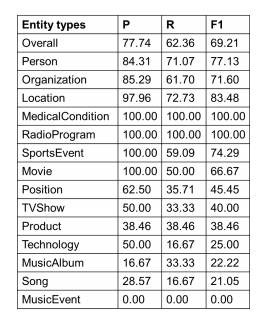
\includegraphics[height=8cm]{Classification_entities}
\caption{The accuracy of the system for extraction and linking.}
%P is the precision, R is the recall and $F_{1}$ is the $F_{1}$-score.} %linking\footnote{\url{http://pages.cs.wisc.edu/~anhai/papers/doctagger-vldb13.pdf, page 8}}}
\label{fig:classification_entities}
\end{figure}

\section{Text Categorization with Encyclopedic Knowledge}
The task of automatic content analysis has many challenges that need to be solved. 

One of the most difficult challenges is how to deal with ambiguous words or phrases. Ambiguous words are words that have more than one meaning, and the meaning is usually found from the other words in the sentence. The problem is that complex sentences and advanced grammer makes it harder for the computer to decide the meaning of a word, hence it also makes it difficult to deide the meaning of the sentence. 
%The task of making the computer understand the content of text has many difficult challenges that most humans won't encounter. Ambiguous words are for example usually not a problem for humans because it is usually easy to use the context to understand the meaning of the word. 
%Computers on the other hand depend on a dictionary or statics about the word to decide the meaning of the word. Complex sentences could also be a problem for computers, advanced grammar for example can make it difficult to interpret the meaning of the sentence.
The paper \emph{Overcoming Brittleness Bottleneck using Wikipedia: Enhancing Text Categorization with Encyclopedic Knowledge} \cite{brittleness} focus on some of these challenges and presents a solution to these. 

Some of these findings are relevant for our project or interesting for further works, hence some solutions to the common ones are mentioned here. 

One of the main problems in  content analysis performed by a computer is to decide the meaning of a word. Humans have a larger background of knowledge and experience which makes it easier to interpret the meaning of a word. Computers depend on either representing documents as bag of words (BOW) or by learning the context of the word by observation. Context is difficult for a computer because it has to decide the number of words that are needed to decide the context of a word, which obviously depends on the word. 

%Ambiguous words are foten understood from the context, but a computer is then either depending on observing the word in a similar context 

%Ambiguous words or sentences are therefore seldom a  problem for humans because the meaning can be found in the context, but a computer could encounter problems with deciding the meaning if the context is unobserved.

The paper presents a text categorization feature to make it easier for the computer to understand the meaning of a word without analysing the context. A feature is a measure for a property of the observation, for instance is number of occurrences a normal feature for each word in the  BOW. If more than one feature measured for an observation are  usually put together as a feature vector for the observation. The feature generator described in the paper takes text fragments as input and maps these to the most relevant Wikipedia articles. The concepts in the relevant articles are used to find new features, which are added to the augmented bag of words. The authors have chosen the feature generator to be a multi-resolution to generate the best relevant Wikipedia concepts, i.e., it generates features at different levels: individual word level, sentence level, paragraph level and for the whole document. This means that there is a large number of features for each document, and these features are useful to understand the content of the document. 

The feature generator depends on  a text classifier that match documents with the most relevant articles of Wikipedia. The classifier starts by manipulating the text into the same form as the encyclopedic articles. This part resembles our categorization problem since we are also interested in linking texts to Wikipedia or information from Wikipedia.  The discussion about ambiguity is also relevant for our problem, where ambiguous words should either be dropped from the keyword list or the computer will have to find the meaning of the words. 


\section{Decoding Wikipedia Categories for Knowledge Acquistion}

We have seen that the catgories contain lots of information about their pages.

This is relevant when we want to map all our Wikipedia cateogires to the desired categories . 

The paper describes ways of finding out about the content of pages based on the name of the cateogires. We could do similar in our project by using some of the same approaches. The \emph{IN} is a useful way to find all categoires .. 



\subsection{Extracting Semantic Relationships between Wikipedia Categories}

\subsubsection{What is the article about?}
Hvordan man kan gjøre Wikipedia søk bedre: Hente semantic informasjon og analysere linker mellom ategoriene. 

Find the type of semantic connections between Wikipedia categories. (sort between weak, average and strong).  Two measures: number of links between pages in two categories, connectivity ratio.

Extracting semantically important relationships: 
goal: emphasize the meaningful relationships between categories and disregard unimportant ones. 


strong relationship: A should conceptually have at least one semantic link to B
average: 50\% of the pages should have semantic links to B
weak: less than 50 \%

Number of links between categories is a good indicator of the level of semantic relationship: number of pages in source category which have at least one link to any page in the target category. 

CONC: Inset: obtained stronger semantic relationships in comparison to outset. 



\subsubsection{What can be added to our solution? How could our solution be better based on their findings?}
If we are able to represent the relationships between Wikipedia categories, we might be able to choose better paths to represent the meaning of the Wikipedia articles. 

We could take advantage of linkage within the documents as well - better know the meaning of the article. 


\subsubsection{Possible quotations}
Pages in Wikipedia are explicitly assigned to one or more \emph{Categories}. 

While most of them are created to provide efficient navitation of the Wikipedia contents, they also represent some semantic relationships between pages and categories. 

Wikipedia forms a signel conntected graph without isolated components or outliers. 



\textbf{Describe the graph: }
Graph: nodes are categories and the edges are hyperlinks. 
--> nodes are categories and the edges are links between categories 





\section{Disambiguation}
\label{sec:disambiguation}

Most people would prefer to interact with their computer in natural language, e.g., search for \emph{"What is computer science?"} rather than \emph{"computer science definition"}. We have already mentioned that the task of understanding natural language is called \emph{Natural Language Processing} (NLP) and is a difficult task because it requires the computer to actually understand the meaning of text. This task is especially difficult because of ambiguity. 

Ambiguity means that there are more than one meaning to a word, phrase or sentence, and disambiguation is the task of finding the correct meaning. There exists many different types of ambiguity \cite[][p.100 and p.466-468]{jurafsky2000speech}% , but our problem is most concerned with 
\begin{itemize}
\item Part-of-speech ambiguity where a part of the sentence is ambiguous. Example: \emph{book} could be either a noun (\emph{hand me that \emph{book}}) or a verb (\emph{\emph{book} that flight}).
\item Structural ambiguity where the structure of the sentence is ambiguous. This can be split into further types
\begin{itemize}
\item Attachment ambiguity where it is not clear how the words are connected together. Example: \emph{We saw the Eiffel tower flying to Paris}.
\item Coordination ambiguity where sets of phrases are joined by conjunction. Example: \emph{Old men and women}.
\end{itemize}
\item Local ambiguity where some part of the sentence is ambiguous even if the whole sentence is not ambiguous. 

%Example: The sentence \emph{book that flight} is not ambiguous, but the word \emph{book} is a local amibugity in the sentence since we can 

\end{itemize}
Many sentences in natural language are complex and combine the different types of ambiguity. This makes it hard for the computer to determine the meaning of the sentence. 


Ambiguous keywords are a problem for our classifier, which means that part-of-speech ambiguity the most relevant for our project. Our solution was to remove all all ambiguous keywords from our dictionary-based classifier, but a good extension for our implementation is to handle disambiguation in a better way. Hence, we have examined some projects for resolving ambiguity:

\begin{enumerate}
\item \emph{Named entity disambiguation by leveraging wikipedia semantic knowledge} \cite{han2009named}. 
\item \emph{Large-scaled named entity disambiguation based on Wikipedia data} \cite{cucerzan2007large}. 
\item \emph{Distributed Representations of Words and Phrases and their compositionality} \cite{mikolov2013distributed}.
\end{enumerate}

\subsubsection{Ambiguous entities}
Project \cite{han2009named} and \cite{cucerzan2007large} encounter the same disambiguation problem as us; entities that have various meanings. The idea of their solution is to measure similarities between occurrences of names and use this to determine whether two occurrences of a specific name represent the same entity. Both projects look through internal hyperlinks in Wikipedia articles and collect all surface forms\footnote{Surface form is defined as full name, acronym, alternative names and spelling variations that occur for an Wikipedia article title} of each article (entity). 



%Another project for solving ambiguous entities is \cite{cucerzan2007large}. This project finds surface forms of entities in a similar way as \cite{han2009named} where they look at hyperlinks between Wikipedia articles, but they also look at titles at the disambiguation pages and the redirecting pages.  


%by looking at the titles of Wikipedia articles, disambiguation pages, titles of redirecting pages and references to the articles from other Wikipedia articles.

In addition, \cite{cucerzan2007large} finds both semantic relations and social relatedness between Wikipedia in the task of determining the meaning of an entity. This is done by studying hyperlinks between them. The combination of these three factors form a way of avoiding ambiguity, since the most likely meaning is set for each Wikipedia article. 
Project \cite{han2009named} solves ambiguity by also looking at titles at the disambiguation pages and the redirecting pages, and represent the Wikipedia entities as vectors in a vector space model. 

The last project studied for solving disambiguation is provided by Google in \cite{mikolov2013distributed}. This project used a different approach, where they created an improved Skip-gram model. All words are represented in a vector space, with semantic and syntactic relationships represented between the words. The training of the Skip-gram model made it possible to determine the meaning of the words based on the semantic relationships to other words within the vector space. 



\end{comment}

% Evaluation of 